\subsection{Contained class set fields}
\label{subsec:library_of_transformations:type_level_transformations:contained_class_set_fields}

\begin{figure}
    \centering
    \begin{subfigure}{0.95\textwidth}
        \centering
        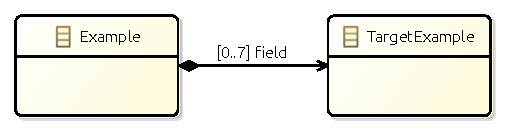
\includegraphics{images/05_library_of_transformations/02_type_level_transformations/10_contained_class_set_fields/contained_class_set_field.pdf}
        \caption{$Tm_{ContainedClassSetField}$ to a class type $.\type{TargetExample}$ with $name = \type{field}$}
        \label{fig:library_of_transformations:type_level_transformations:contained_class_set_fields:visualisation:ecore}
    \end{subfigure}
    \\
    \begin{subfigure}{0.95\textwidth}
        \centering
        % To use this figure in your LaTeX document
% import the package groove/resources/groove2tikz.sty
%
\begin{tikzpicture}[scale=\tikzscale,name prefix=test-]
\node[type_node] (n0) at (3.125, -0.945) {\ml{\textbf{Example}}};
\node[type_node] (n1) at (5.040, -0.950) {\ml{\textbf{TargetExample}}};

\path[basic_edge, composite](n0.east |- 5.040, -0.950) -- node[lab] {\ml{field}} (n1) ;
\end{tikzpicture}

        \caption{$TG_{ContainedClassSetField}$ to a class type $\type{TargetExample}$ with $name = \type{field}$}
        \label{fig:library_of_transformations:type_level_transformations:contained_class_set_fields:visualisation:groove}
    \end{subfigure}
    \caption{Visualisation of the transformation of a containment field typed by a set of a proper class type}
    \label{fig:library_of_transformations:type_level_transformations:contained_class_set_fields:visualisation}
\end{figure}

In this section, the transformation of a containment field typed by a set of a proper class type is shown. This transformation defines a field which has a value a set of objects of a specified class type, that is not nullable. Furthermore, the objects referenced by the field are contained by the source class. First, the Ecore type model is defined.

\begin{defin}[Type model $Tm_{ContainedClassSetField}$]
\label{defin:library_of_transformations:type_level_transformations:contained_class_set_fields:tmod_contained_class_set_field}
Let $Tm_{ContainedClassSetField}$ be the type model containing a regular class with identifier $classtype$. Then $Tm_{ContainedClassSetField}$ defines a field named $name$ with type $containedtype$, in which $containedtype$ is the identifier of another class type in $Tm_{ContainedClassSetField}$. Furthermore, define $mul$ to be a valid multiplicity for the field $name$. $Tm_{ContainedClassSetField}$ is defined as:
\begin{align*}
Class =\ &\{classtype, containedtype\} \\
Enum =\ &\{\} \\
UserDataType =\ &\{\} \\
Field =\ &\{(classtype, name)\} \\
\mathrm{FieldSig} =\ &\begin{cases}
    (f, ((\type{setof}, !containedtype), mul)) &\mathrm{if}\ f \in Field_{Tm_{ContainedClassSetField}}
\end{cases} \\
EnumValue =\ &\{\} \\
Inh =\ &\{\} \\
Prop =\ &\{(\type{containment}, (classtype, name))\} \\
Constant =\ &\{\} \\
\mathrm{ConstType} =\ &\{\}
\end{align*}
\isabellelref{tmod_contained_class_set_field}{Ecore-GROOVE-Mapping-Library.ContainedClassSetField}
\end{defin}

\begin{thm}[Correctness of $Tm_{ContainedClassSetField}$]
\label{defin:library_of_transformations:type_level_transformations:contained_class_set_fields:tmod_contained_class_set_field_correct}
$Tm_{ContainedClassSetField}$ (\cref{defin:library_of_transformations:type_level_transformations:contained_class_set_fields:tmod_contained_class_set_field}) is a consistent type model in the sense of \cref{defin:formalisations:ecore_formalisation:type_models:type_model_consistency}.
\isabellelref{tmod_contained_class_set_field_correct}{Ecore-GROOVE-Mapping-Library.ContainedClassSetField}
\end{thm}

A visual representation of $Tm_{ContainedClassSetField}$ with field name $\type{field}$ on class $.\type{Example}$ can be seen in \cref{fig:library_of_transformations:type_level_transformations:contained_class_set_fields:visualisation:ecore}. In this example, $\type{field}$ references a class of $.\type{TargetExample}$. Please note that the multiplicity $0..7$ has been chosen here as an example, any valid multiplicity could have been used. Also notice that the field is in fact a containment relation. The correctness proof of $Tm_{ContainedClassSetField}$ is more involved, it is not included here for conciseness. It can be found within the validated Isabelle proofs.

In order to make composing transformation functions possible, $Tm_{ContainedClassSetField}$ should be compatible with the type model it is combined with.

\begin{thm}[Correctness of $\mathrm{combine}(Tm, Tm_{ContainedClassSetField})$]
\label{defin:library_of_transformations:type_level_transformations:contained_class_set_fields:tmod_contained_class_set_field_combine_correct}
Assume a type model $Tm$ that is consistent in the sense of \cref{defin:formalisations:ecore_formalisation:type_models:type_model_consistency}. Then $Tm$ is compatible with $Tm_{ContainedClassSetField}$ (in the sense of \cref{defin:transformation_framework:type_models_and_type_graphs:combining_type_models:compatibility}) if:
\begin{itemize}
    \item The class type on which the field is defined, $classtype$, is already an existing class in $Tm$;
    \item The class type which the field targets, $containedtype$, is already an existing class in $Tm$;
    \item The field named $name$ is not already a field on $classtype$ in $Tm$;
    \item The multiplicity $mul$ is valid.
\end{itemize}
\isabellelref{tmod_contained_class_set_field_combine_correct}{Ecore-GROOVE-Mapping-Library.ContainedClassSetField}
\end{thm}

\begin{proof}
Use \cref{defin:transformation_framework:type_models_and_type_graphs:combining_type_models:tmod_combine_merge_correct}. It is possible to show that all assumptions hold. Now we have shown that $\mathrm{combine}(Tm, Tm_{ContainedClassSetField})$ is consistent in the sense of \cref{defin:formalisations:ecore_formalisation:type_models:type_model_consistency}.
\end{proof}

The definitions and theorems for defining a data field within Ecore are now complete. 

\subsubsection{Encoding as edge type}

Like the previous encodings of fields, an edge type in GROOVE will be used as encoding for the field. The field is transformed into an edge type from the encoded class type to the encoded target type. Furthermore, the edge type will be a containment edge, to support the fact that the target nodes are contained by the source nodes. The encoding corresponding to $Tm_{ContainedClassSetField}$ can then be represented as $TG_{ContainedClassSetField}$, defined in the following definition:

\begin{defin}[Type graph $TG_{ContainedClassSetField}$]
\label{defin:library_of_transformations:type_level_transformations:contained_class_set_fields:tg_contained_class_set_field_as_edge_type}
Let $TG_{ContainedClassSetField}$ be the type graph containing a node type which encodes the class type $classtype$. Furthermore, define an edge type from $classtype$ named $name$. This edge type targets a node of $containedtype$. Finally, define multiplicity $mul$ to be  $TG_{ContainedClassSetField}$ is defined as:
\begin{align*}
NT =\ &\{\mathrm{ns\_\!to\_\!list}(classtype), \mathrm{ns\_\!to\_\!list}(containedtype)\} \\
ET =\ &\{(\mathrm{ns\_\!to\_\!list}(classtype), \langle name \rangle, \mathrm{ns\_\!to\_\!list}(containedtype))\} \\
\!\!\sqsubseteq\ =\ &\{( \mathrm{ns\_\!to\_\!list}(classtype), \mathrm{ns\_\!to\_\!list}(classtype) ),\\&( \mathrm{ns\_\!to\_\!list}(containedtype), \mathrm{ns\_\!to\_\!list}(containedtype) )\} \\
abs =\ &\{\} \\
\mathrm{mult}(e) =\ &\begin{cases}
    (0..1, mul) &\mathrm{if}\ e \in \{(\mathrm{ns\_\!to\_\!list}(classtype), \langle name \rangle, \mathrm{ns\_\!to\_\!list}(containedtype))\}
\end{cases} \\
contains =\ &\{(\mathrm{ns\_\!to\_\!list}(classtype), \langle name \rangle, \mathrm{ns\_\!to\_\!list}(containedtype))\}
\end{align*}
\isabellelref{tg_contained_class_set_field_as_edge_type}{Ecore-GROOVE-Mapping-Library.ContainedClassSetField}
\end{defin}

\begin{thm}[Correctness of $TG_{ContainedClassSetField}$]
\label{defin:library_of_transformations:type_level_transformations:contained_class_set_fields:tg_contained_class_set_field_as_edge_type_correct}
$TG_{ContainedClassSetField}$ (\cref{defin:library_of_transformations:type_level_transformations:contained_class_set_fields:tg_contained_class_set_field_as_edge_type}) is a valid type graph in the sense of \cref{defin:formalisations:groove_formalisation:type_graphs:type_graph_validity}.
\isabellelref{tg_contained_class_set_field_as_edge_type_correct}{Ecore-GROOVE-Mapping-Library.ContainedClassSetField}
\end{thm}

A visual representation of $TG_{ContainedClassSetField}$ with edge name $\type{field}$ on node type $\type{Example}$ can be seen in \cref{fig:library_of_transformations:type_level_transformations:contained_class_set_fields:visualisation:groove}. Like the previous example, $\type{field}$ references the $.\type{TargetExample}$ class, but in this case the encoded node type of $\type{TargetExample}$. Furthermore, it is visable that the introduced edge type for the field is indeed a containment edge. The correctness proof of $TG_{ContainedClassSetField}$ is more involved, it is not included here for conciseness. It can be found within the validated Isabelle proofs.

In order to make composing transformation functions possible, $TG_{ContainedClassSetField}$ should be compatible with the type graph it is combined with.

\begin{thm}[Correctness of $\mathrm{combine}(TG, TG_{ContainedClassSetField})$]
\label{defin:library_of_transformations:type_level_transformations:contained_class_set_fields:tg_contained_class_set_field_as_edge_type_combine_correct}
Assume a type graph $TG$ that is valid in the sense of \cref{defin:formalisations:groove_formalisation:type_graphs:type_graph_validity}. Then $TG$ is compatible with $TG_{ContainedClassSetField}$ (in the sense of \cref{defin:transformation_framework:type_models_and_type_graphs:combining_type_graphs:compatibility}) if:
\begin{itemize}
    \item The node types of the encoded class types in $TG_{ContainedClassSetField}$ are already node types in $TG$.
    \item The node type of the encoded class type in $TG_{ContainedClassSetField}$ does not already have an edge type with the same name as the field in $TG$;
    \item The multiplicity $mul$ is valid.
\end{itemize}
\isabellelref{tg_contained_class_set_field_as_edge_type_combine_correct}{Ecore-GROOVE-Mapping-Library.ContainedClassSetField}
\end{thm}

\begin{proof}
Use \cref{defin:transformation_framework:type_models_and_type_graphs:combining_type_graphs:tg_combine_merge_correct}. It is possible to show that all assumptions hold. Now we have shown that $\mathrm{combine}(TG, TG_{ContainedClassSetField})$ is valid in the sense of \cref{defin:formalisations:groove_formalisation:type_graphs:type_graph_validity}.
\end{proof}

The next definitions define the transformation function from $Tm_{ContainedClassSetField}$ to $TG_{ContainedClassSetField}$:

\begin{defin}[Transformation function $f_{ContainedClassSetField}$]
\label{defin:library_of_transformations:type_level_transformations:contained_class_set_fields:tmod_contained_class_set_field_to_tg_contained_class_set_field_as_edge_type}
The transformation function $f_{ContainedClassSetField}(Tm)$ is defined as:
\begin{align*}
NT =\ &\{\mathrm{ns\_\!to\_\!list}(c) \mid c \in Class_{Tm}\}\\
ET =\ &\{(\mathrm{ns\_\!to\_\!list}(c), \langle f \rangle, \mathrm{ns\_\!to\_\!list}(containedtype)) \mid (c, n) \in Field_{Tm} \} \\
\!\!\sqsubseteq\ =\ &\{( \mathrm{ns\_\!to\_\!list}(c), \mathrm{ns\_\!to\_\!list}(c) ) \mid c \in Class_{Tm} \} \\
abs =\ &\{\} \\
\mathrm{mult} =\ &\begin{cases}
    (0..1, mul) &\mathrm{if}\ e \in \{(\mathrm{ns\_\!to\_\!list}(c), \langle f \rangle, \mathrm{ns\_\!to\_\!list}(containedtype)) \mid (c, n) \in Field_{Tm} \}
\end{cases} \\
contains =\ &\{(\mathrm{ns\_\!to\_\!list}(c), \langle f \rangle, \mathrm{ns\_\!to\_\!list}(containedtype)) \mid (c, n) \in Field_{Tm} \}
\end{align*}
\isabellelref{tmod_contained_class_set_field_to_tg_contained_class_set_field_as_edge_type}{Ecore-GROOVE-Mapping-Library.ContainedClassSetField}
\end{defin}

\begin{thm}[Correctness of $f_{ContainedClassSetField}$]
\label{defin:library_of_transformations:type_level_transformations:contained_class_set_fields:tmod_contained_class_set_field_to_tg_contained_class_set_field_as_edge_type_func}
$f_{ContainedClassSetField}(Tm)$ (\cref{defin:library_of_transformations:type_level_transformations:contained_class_set_fields:tmod_contained_class_set_field_to_tg_contained_class_set_field_as_edge_type}) is a valid transformation function in the sense of \cref{defin:transformation_framework:type_models_and_type_graphs:combining_transformation_functions:transformation_function_type_model_type_graph} transforming $Tm_{ContainedClassSetField}$ into $TG_{ContainedClassSetField}$.
\isabellelref{tmod_contained_class_set_field_to_tg_contained_class_set_field_as_edge_type_func}{Ecore-GROOVE-Mapping-Library.ContainedClassSetField}
\end{thm}

The proof of the correctness of $f_{ContainedClassSetField}$ will not be included here. Instead, it can be found in the validated Isabelle theories.

Finally, to complete the transformation, the transformation function that transforms $TG_{ContainedClassSetField}$ into $Tm_{ContainedClassSetField}$ is defined:

\begin{defin}[Transformation function $f'_{ContainedClassSetField}$]
\label{defin:library_of_transformations:type_level_transformations:contained_class_set_fields:tg_contained_class_set_field_as_edge_type_to_tmod_contained_class_set_field}
The transformation function $f'_{ContainedClassSetField}(TG)$ is defined as:
\begin{align*}
Class =\ &\{\mathrm{list\_\!to\_\!ns}(n) \mid n \in NT_{TG} \} \\
Enum =\ &\{\} \\
UserDataType =\ &\{\} \\
Field =\ &\{(\mathrm{list\_\!to\_\!ns}(\mathrm{src}(e)), l) \mid e \in ET_{TG} \land \langle l \rangle = \mathrm{lab}(e) \} \\
\mathrm{FieldSig} =\ &\begin{cases}
    (f, ((\type{setof}, !containedtype), mul)) &\mathrm{if}\ f \in \{(\mathrm{list\_\!to\_\!ns}(\mathrm{src}(e)), l) \mid e \in ET_{TG}\ \land\\&\qquad\quad \langle l \rangle = \mathrm{lab}(e) \} 
\end{cases} \\
EnumValue =\ &\{\} \\
Inh =\ &\{\} \\
Prop =\ &\{(\type{containment}, (\mathrm{list\_\!to\_\!ns}(\mathrm{src}(e)), l)) \mid e \in ET_{TG} \land \langle l \rangle = \mathrm{lab}(e) \} \\
Constant =\ &\{\} \\
\mathrm{ConstType} =\ &\{\}
\end{align*}
\isabellelref{tg_contained_class_set_field_as_edge_type_to_tmod_contained_class_set_field}{Ecore-GROOVE-Mapping-Library.ContainedClassSetField}
\end{defin}

\begin{thm}[Correctness of $f'_{ContainedClassSetField}$]
\label{defin:library_of_transformations:type_level_transformations:contained_class_set_fields:tg_contained_class_set_field_as_edge_type_to_tmod_contained_class_set_field_func}
$f'_{ContainedClassSetField}(TG)$ (\cref{defin:library_of_transformations:type_level_transformations:contained_class_set_fields:tg_contained_class_set_field_as_edge_type_to_tmod_contained_class_set_field}) is a valid transformation function in the sense of \cref{defin:transformation_framework:type_models_and_type_graphs:combining_transformation_functions:transformation_function_type_graph_type_model} transforming $TG_{ContainedClassSetField}$ into $Tm_{ContainedClassSetField}$.
\isabellelref{tg_contained_class_set_field_as_edge_type_to_tmod_contained_class_set_field_func}{Ecore-GROOVE-Mapping-Library.ContainedClassSetField}
\end{thm}

Once more, the correctness proof is not included here but can be found in the validated Isabelle proofs of this thesis.